% !TEX root = saveliev_physics_general_course_2.tex
%!TEX TS-program = pdflatex
%!TEX encoding = UTF-8 Unicode


\chapter[CONDUCTORS IN AN ELECTRIC FIELD]{CONDUCTORS IN AN ELECTRIC \\FIELD}\label{chap:3}
\chaptermark{VẬT DẪN TRONG ĐIỆN TRƯỜNG}


\section{Cân bằng điện tích trên vật dẫn}\label{sec:3_1}

Các hạt mang điện trong vật dẫn có thể chuyển động dưới tác dụng của một lực rất nhỏ. Do đó, phải có các điều kiện sau đây để các điện tích trên vật dẫn cân bằng:
\begin{enumerate}[1.]
    \item Cường độ trường tại mọi nơi bên trong vật dẫn phải bằng không:
    \begin{equation}\label{eq:3_1}
        \vec{E} = 0.
    \end{equation}

    \noindent
    Phù hợp với \eqn{1_41}, điều này chỉ ra rằng điện thế bên trong vật dẫn phải là hằng số ($\varphi=\text{constant}$).

    \item Điện trường trên bề mặt vật dẫn phải hướng dọc theo pháp tuyến bề mặt tại mọi điểm:
    \begin{equation}\label{eq:3_2}
        \vec{E} = \vec{E}_n.
    \end{equation}

    \noindent
    Kết quả là, khi các điện tích ở trạng thái cân bằng, bề mặt vật dẫn là một mặt đẳng thế.
\end{enumerate}

Nếu một điện tích $q$ được truyền cho một vật dẫn, điện tích sẽ phân bố sao cho đạt được điều kiện cân bằng. Ta hãy tưởng tượng một bề mặt đóng kín tùy ý bị giới hạn hoàn toàn trong một vật. Khi các điện tích cân bằng, không có điện trường tại mọi điểm trong vật dẫn; do đó, thông lượng của vector điện dịch qua bề mặt biến mất. Theo định lý Gauss, tổng điện tích bên trong bề mặt cũng phải bằng không. Điều này đúng cho bề mặt có kích thước bất kỳ được sắp xếp tùy ý bên trong vật dẫn. Từ đó, khi cân bằng, không thể có điện tích dư nào bên trong vật dẫn---tất cả chúng sẽ được phân bố trên bề mặt vật dẫn với mật độ nhất định $\sigma$.

Vì không có điện tích dư trong vật dẫn ở trạng thái cân bằng, việc loại bỏ vật chất từ một thể tích bên trong vật dẫn sẽ không có ảnh hưởng gì đến phân bố cân bằng của điện tích. Do đó, một điện tích dư sẽ được phân bố trên một vật dẫn rỗng giống như một vật dẫn đặc, tức là, dọc theo mặt ngoài của nó. Không có điện tích dư phân bố trên bề mặt của một cái hốc ở trạng thái cân bằng. Kết luận này tuân theo thức tế rằng các điện tích nguyên tố tạo thành điện tích đã cho $q$ đẩy lẫn nhau và, kết quả là, có xu hướng chiếm các vị trí xa nhau nhất.

Tưởng tượng một mặt trụ nhỏ tạo bởi pháp tuyến của bề mặt một vật dẫn và độ lớn đáy $\deriv{S}$, một đáy bên trong và cái còn lại bên ngoài vật dẫn (\fig{3_1}). Thông lượng của vector điện dịch qua phần trong của bề mặt bằng không vì $\vec{E}$ và, do đó, $\vec{D}$ không có trong vật dẫn. Bên ngoài vật dẫn ở gần nó, cường độ trường $\vec{E}$ hướng dọc theo pháp tuyến bề mặt. Do đó, đối với mặt bên hình trụ nhô ra ngoài, $D_n=0$, và với đáy ngoài $D_n=D$ (đáy ngoài được cho là rất gần bề mặt vật dẫn). Do đó, thông lượng qua bề mặt là $D\,\deriv{S}$, với $D$ là giá trị của điện dịch ở sát bề mặt vật dẫn. Hình trụ chưa một điện tích $\sigma\,\deriv{S}$ ($\sigma$ là mật độ điện mặt tại điểm cho trước trên bề mặt vật dẫn).

\begin{figure}[!htb]
	\begin{center}
		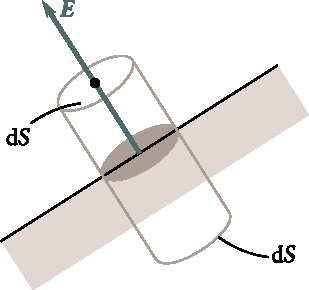
\includegraphics[scale=1]{figures/ch_03/fig_3_1.pdf}
		\caption[]{}
		\label{fig:3_1}
	\end{center}
	\vspace{-0.8cm}
\end{figure}

Áp dụng định lý Gauss, ta có $D\,\deriv{S}=\sigma\,\deriv{S}$, tức là, $D=\sigma$. Do đó ta thấy rằng cường độ trường gần bề mặt vật dẫn là
\begin{equation}\label{eq:3_3}
    E = \frac{\sigma}{\varepsilon_0\varepsilon}
\end{equation}

\noindent
với $\varepsilon$ là hằng số điện môi của môi trường xung quanh vật dẫn [so sánh với \eqn{1_123} nhận được cho trường hợp khi $\varepsilon=1$].

Ta hãy xem xét trường tạo ra bởi vật dẫn tích điện trong \fig{3_2}. Tại khoảng cách rất lớn từ vật dẫn, mặt đẳng thế có dạng hình cầu đặc trưng của một điện tích điểm (do thiếu không gian, một mặt cầu được chỉ ra trong hình tại khoảng cách nhỏ từ vật dẫn; các đường nét đứt là đường sức trường). Khi ta tiếp cận vật dẫn, các mặt đẳng thế trở nên càng lúc càng giống bề mặt vật dẫn, cũng là một mặt đẳng thế. Gần mặt phân cách, các mặt đẳng thế dày đặc hơn, từ đó, cường độ trường cũng mạnh hơn ở đây. Do đó, mật độ điện tích trên mặt phân cách là đặc biệt lớn [xem \eqn{3_3}]. Ta có thể đi đến cùng một kết luận bằng cách xem xét rằng do lực đẩy lẫn nhau giữa chúng, điện tích có xu hướng chiếm các vị trí xa nhau nhất có thể.

\begin{figure}[!htb]
	\begin{minipage}[t]{0.48\linewidth}
		\begin{center}
			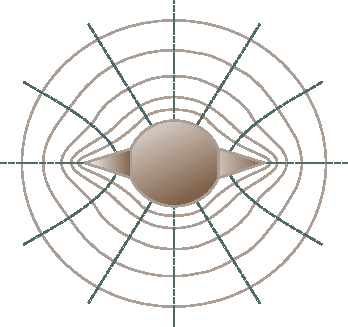
\includegraphics[scale=1]{figures/ch_03/fig_3_2.pdf}
			\caption[]{}
			\label{fig:3_2}
		\end{center}
	\end{minipage}
	\hfill{ }%space{-0.05cm}
	\begin{minipage}[t]{0.48\linewidth}
		\begin{center}
			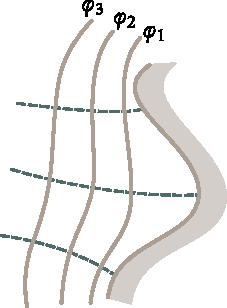
\includegraphics[scale=1]{figures/ch_03/fig_3_3.pdf}
			\caption[]{}
			\label{fig:3_3}
		\end{center}
	\end{minipage}
\vspace{-0.4cm}
\end{figure}

Gần chỗ lõm của vật dẫn, các mặt đẳng thế có mật độ thấp hơn (xem \fig{3_3}). Do đó, cường độ trường và mật độ điện tích tại các điểm này sẽ nhỏ hơn. Nói chung, mật độ điện tích với một điện thế xác định của vật dẫn được xác định bởi độ cong của bề mặt---nó tăng với sự gia tăng độ cong dương (lồi) và giảm dần với độ tăng độ cong âm (lõm). Mật độ điện tích đặc biệt lớn tại các điểm nhọn. Kết quả là, cường độ trường gần các điểm này có thể lớn tới nỗi làm ion hóa các phân tử khí xung quanh vật dẫn. Ion trái dấu $q$ bị hút về vật dẫn và trung hòa điện tích của nó. Ion cùng dấu $q$ bắt đầu di chuyển ra xa vật dẫn, mang theo các phân tử khí trung hòa. Kết quả là một chuyển động đáng chú ý của khí gọi là gió điện. Điện tích của vật dẫn giảm dần, nó chảy ra khỏi điểm, như nó đã từng, và bị mang đi bởi gió. Hiện tượng này do đó được gọi là sự phát ra điện tích từ một điểm.

\section{Vật dẫn trong điện trường}\label{sec:3_2}

Khi một vật dẫn không tích điện được đưa vào một điện trường, các hạt mang điện chuyển động: các hạt dương theo hướng của vector $\vec{E}$, những hạt âm theo hướng ngược lại. Kết quả là, các điện tích trái dấu gọi là \textbf{điện tích cảm ứng} xuất hiện tại các đầu vật dẫn (\fig{3_4}, các đường nét đứt mô tả các đường sức trường ngoài). Trường của các điện tích này hướng ngược lại trường ngoài. Do đó, sự tích tụ các điện tích tại các đầu vật dẫn làm suy yếu trường bên trong nó. Các hạt mang điện sẽ được phân bố lại cho tới khi các điều kiện \eqref{eq:3_1} và \eqref{eq:3_2} được thiết lập, tức là, cho tới khi cường độ trường trong vật dẫn biến mất và các đường sức trường bên ngoài vật dẫn vuông góc với bề mặt của nó (xem \fig{3_4}). Do đó, một vật dẫn trung hòa được đưa vào một điện trường làm gián đoạn một phần đường sức---chúng kết thúc trên các điện tích cảm ứng âm và bắt đầu lại trên các điện tích cảm ứng dương.

\begin{figure}[!htb]
	\begin{center}
		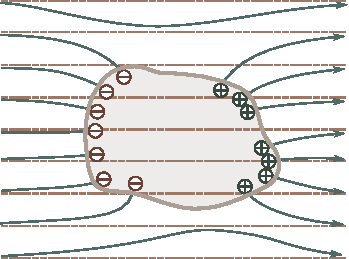
\includegraphics[scale=1]{figures/ch_03/fig_3_4.pdf}
		\caption[]{}
		\label{fig:3_4}
	\end{center}
	\vspace{-0.8cm}
\end{figure}

Các điện tích cảm ứng tự phân bố trên mặt ngoài vật dẫn. Nếu vật dẫn chứa một khoảng trống, thì khi phân bố cân bằng các điện tích cảm ứng, trường bên trong nó biến mất. Che chắn tĩnh điện dựa trên hiện tượng này. Nếu một dụng cụ được bảo vệ khỏi ảnh hưởng của trường ngoài, nó được bao quanh bởi một bề mặt dẫn điện. Trường ngoài được bù trừ bên trong bề mặt bởi các điện tích cảm ứng xuất hiện trên bề mặt của nó. Một bề mặt như vậy cũng hoạt động khá tốt nếu nó được làm không đặc, nhưng ở dạng mạng lưới dày đặc.

\section{Điện dung}\label{sec:3_3}

Một điện tích $q$ truyền cho một vật dẫn được phân bố trên bề mặt vật dẫn làm cho cường độ trường bên trong vật dẫn biến mất. Phân bố như vậy là duy nhất. Do đó, nếu ta truyền cho một vật dẫn đã mang điện tích $q$ một điện tích cùng độ lớn, thì điện tích thứ hai phải phân bố trên vật dẫn chính xác giống như cách của điện tích thứ nhất. Nếu không thì, điện tích sẽ tạo ra bên trong vật dẫn một trường khác không. Ta phải chú ý rằng điều này chỉ đúng cho một vật dẫn ở xa các vật thể khác (một vật dẫn cô lập). Nếu các vật thể khác ở gần vật dẫn, việc truyền cho phần sau một lượng điện tích mới sẽ tạo ra sự thay đổi trong sự phân cực của các vật thể này hoặc điện tích cảm ứng trên chúng. Kết quả là, sự giống nhau trong phân bố của các lượng điện tích khác nhau sẽ bị phá vỡ.

Do đó, các điện tích khác nhau về độ lớn phân bố trên một vật dẫn cô lập theo một cách tương tự nhau (tỷ lệ của mật độ điện tích tại hai điểm tùy ý trên bề mặt vật dẫn với bất kì độ lớn điện tích nào cũng sẽ như nhau). Do đó, điện thế của một vật dẫn cô lập tỷ lệ thuận với điện tích trên nó. Đúng vậy, sự tăng điện tích một số lần nhất định dẫn đến cường độ trường tại mọi điểm trong không gian xung quanh vật dẫn tăng cùng một số lần. Theo đó, công cần thiết để chuyển một điện tích nguyên tố từ vô cực đến bề mặt của một vật dẫn, tức là, điện thế của vật dẫn, tăng cùng số lần. Do đó, với một vật dẫn cô lập
\begin{equation}\label{eq:3_4}
    q = C \varphi.
\end{equation}

\noindent
Hằng số tỷ lệ $C$ giữa điện thế và điện tích gọi là \textbf{điện dung}. Từ \eqn{3_4}, ta có
\begin{equation}\label{eq:3_5}
    C = \frac{q}{\varphi}.
\end{equation}

\noindent
Theo \eqn{3_5}, điện dung về mặt số học bằng với điện tích truyền cho vật dẫn tăng điện thế nó lên một đơn vị.

Ta hãy tính điện thế của một quả cầu tích điện bán kính $R$. Mối liên hệ giữa hiệu điện thế và cường độ trường cho bởi \eqn{1_45}. Do đó, ta có thể tìm điện thế của quả cầu $\varphi$ bằng cách tích phân \eqn{2_41} theo $r$ từ $R$ tới $\infty$ (ta giả sử rằng điện thế tại vô cực là không):
\begin{equation}\label{eq:3_6}
    \varphi = \frac{1}{4\pi\varepsilon_0} \int_0^{\infty} \frac{q}{\varepsilon r^2}\, \deriv{r} = \frac{1}{4\pi\varepsilon_0} \frac{q}{\varepsilon R}.
\end{equation}

\noindent
So sánh Eqs. \eqref{eq:3_5} và \eqref{eq:3_6}, ta tìm được điện dung của một quả cầu cô lập bán kính $R$ nhúng trong chất điện môi vô hạn đồng nhất có hằng sô điện môi $\varepsilon$ là
\begin{equation}\label{eq:3_7}
    C = 4\pi\varepsilon_0 \varepsilon R.
\end{equation}

Đơn vị của điện dung là điện dung của một vật dẫn mà điện thế của nó thay đổi \SI{1}{\volt} khi một điện tích \SI{1}{\coulomb} truyền cho nó. Đơn vị này của điện dung gọi là \textbf{farad} (\si{\faraday}).
Trong hệ Gauss, công thức của điện dung một quả cầu cô lập có dạng
\begin{equation}\label{eq:3_8}
    C = \varepsilon R.
\end{equation}

\noindent
Vì $\varepsilon$ là một đại lượng không thứ nguyên, điện dung xác định bởi \eqn{3_8} có thứ nguyên của độ dài. Đơn vị của điện dung là điện dung của một quả cầu cô lập với bán kính \SI{1}{\centi\metre} trong chân không. Đơn vị này của điện dung gọi là \textbf{centimetre}. Theo \eqn{3_5},
\begin{equation}\label{eq:3_9}
    \SI{1}{\faraday} = \frac{\SI{1}{\coulomb}}{\SI{1}{\volt}} = \frac{\num{3e9}{\cgse{C}}}{1/300} = \SI{9e11}{\centi\metre}.
\end{equation}

Một quả cầu cô lập có bán kính \SI{9e11}{\centi\metre}, tức là, bán kính gấp $1500$ lần bán kính trái đất, sẽ có điện dung \SI{1}{\faraday}. Do đó, ta có thể thấy Farad là một đơn vị rất lớn. Vì lí do này, các ước của farad thường được sử dụng---millifarad (\si{\milli\faraday}), microfarad (\si{\micro\faraday}), nanofarad (\si{\nano\faraday}), và picofarad (\si{\pico\faraday}) (see Vol. I, Table 3.1).

\section{Tụ điện}\label{sec:3_4}

Vật dẫn cô lập có điện dung nhỏ. Thậm chí một quả cầu có kích thước bằng trái đất cũng có điện dung chỉ \SI{700}{\micro\faraday}. Tuy nhiên, trong thực tế cần phải có các thiết bị có điện thế thấp so với các vật thể xung quanh sẽ tích trữ lượng điện tích đáng kể (tức là, có ``sức chứa'' điện tích lớn). Thiết bị như vậy, gọi là \textbf{tụ điện}, dựa trên thực tế rằng điện dung của một vật dẫn tăng lên khi các vật thể khác được đưa lại gần nó. Điều này là do dưới tác dụng của trường được thiết lập bởi vật dẫn mang điện, điện tích cảm ứng (trên vật dẫn) hoặc liên kết (trên điện môi) xuất hiện trên vật thể mang nó. Các điện tích trái dấu với điện tích $q$ của vật dẫn sẽ gần với vật dẫn hơn các điện tích cùng dấu với $q$ và, kết quả là, sẽ có ảnh hưởng lớn hơn lên điện thế của nó. Do đó, khi một vật được mang lại gần một vật dẫn tích điện, điện thế của vật dẫn giảm dần giá trị tuyệt đối. Theo \eqn{3_5}, điều này làm tăng điện dung của vật dẫn.

Tụ điện được làm ở dạng hai vật dẫn đặt gần nhau. Các vật dẫn tạo thành một tụ điện gọi là \textbf{bản} của nó. Để tránh các vật thể bên ngoài làm ảnh hưởng điện dung của một tụ điện, các bản được định hình và sắp xếp tương đối với nhau sao cho trường tạo bởi các điện tích tích tụ trên nó tập trung bên trong vật dẫn. Điều kiện này được thỏa mãn (xem \sect{1_14}) bởi hai bản được sắp xếp gần nhau, hai hình trụ đồng trục, và hai quả cầu đồng tâm. Do đó, ta thường gặp tụ điện bản song song (mặt phẳng), trụ, và cầu. Vì trường bị giam cầm bên trong tụ điện, các đường điện dịch bắt đầu trên một bản và kết thúc ở bản còn lại. Kết quả là, các điện tích bên ngoài được tạo ra trên các bản có cùng độ lớn và trái dấu nhau.

Đặc tính cơ bản của một tụ điện là điện dung của nó, được hiểu là đại lượng tỷ lệ thuận với điện tích $q$ và tỷ lệ nghịch với hiệu điện thế giữa các bản:
\begin{equation}\label{eq:3_10}
    C = \frac{q}{\varphi_1 - \varphi_2}.
\end{equation}

Hiệu điện thế $\varphi_1-\varphi_2$ được gọi là \textbf{điện áp} giữa các điểm liên quan\footnote{Một định nghĩa tổng quát hơn của đại lượng gọi là điện áp sẽ được đưa ra ở \sect{5_3} [see \eqn{5_18}].}. Ta sẽ sử dụng ký hiệu $U$ để chỉ điện áp. Từ đó, \eqn{3_10} có thể được viết như sau:
\begin{equation}\label{eq:3_11}
    C = \frac{q}{U}.
\end{equation}

\noindent
Ở đây, $U$ là điện áp giữa các bản.

Điện dung tụ điện được đo trong cùng đơn vị như điện dung của vật dẫn cô lập (xem phần trước).

Độ lớn của điện dung được xác định bởi dạng hình học của tụ điện (hình dạng và kích thước của các bản và khoảng cách tách biệt giữa chúng), và cũng bởi đặc tính điện môi của môi trường lấp đầy không gian giữa các bản. Ta hãy tìm phương trình cho điện dung của tụ điện phẳng. Nếu diện tích của bản là $S$ và điện tích trên nó là $q$, thì cường độ trường giữa các bản là
\begin{equation*}
    E = \frac{\sigma}{\varepsilon_0 \varepsilon} = \frac{q}{\varepsilon_0 \varepsilon S}
\end{equation*}

\noindent
[xem Eqs. \eqref{eq:1_121} và \eqref{eq:2_33}; $\varepsilon$ là hằng số điện môi của môi trường lấp đầy khoảng trống giữa các bản].

Phù hợp với \eqn{1_45}, hiệu điện thế giữa các bản là
\begin{equation*}
    \varphi_1 - \varphi_2 = E d = \frac{q d}{\varepsilon_0 \varepsilon S}.
\end{equation*}

\noindent
Từ đó, với điện dung của một tụ phẳng, ta có
\begin{equation}\label{eq:3_12}
    C = \frac{\varepsilon_0 \varepsilon S}{d}
\end{equation}

\noindent
với $S$ là diện tích của một bản, $d$ là khoảng cách giữa các bản, và $\varepsilon$ là hằng số điện môi của chất lấp đầy không gian giữa hai bản.

Cần phải chú ý rằng độ chính xác trong xác định điện dung của một tụ phẳng thực bằng \eqn{3_12} càng lớn, khoảng cách $d$ khi so sánh với kích thước của các bản càng nhỏ.

Có thể thấy từ \eqn{3_12} rằng thứ nguyên của hằng số điện $\varepsilon_0$ bằng với thứ nguyên của điện dung chia cho độ dài. Do đó, $\varepsilon_0$ được đo bằng farad trên mét [xem \eqn{1_12}].

Nếu ta bỏ qua sự phân tán của trường gần cạnh bản, ta có thể dễ dàng nhận được phương trình sau cho điện dung của một tụ trụ:
\begin{equation}\label{eq:3_13}
    C = \frac{2\pi\varepsilon_0\varepsilon l}{\ln\parenthesis{\dfrac{R_2}{R_1}}}
\end{equation}

\noindent
với $l$ là độ dài của tụ, $R_1$ và $R_2$ là bán kính bản trong và ngoài.

Độ chính xác trong xác định điện dung của một tụ điện bằng \eqn{3_13} càng lớn, khoảng cách giữa các bản $d=R_2-R_1$ khi so sánh với $l$ và $R_1$ càng nhỏ.

Điện dung của một tụ cầu là
\begin{equation}\label{eq:3_14}
    C = 4\pi\varepsilon_0\varepsilon \parenthesis{\frac{R_1 R_2}{R_2 - R_1}}
\end{equation}

\noindent
với $R_1$ và $R_2$ là bán kính bản trong và ngoài.

Ngoài điện dung, mọi tụ điện được đặc trưng bằng điện áp cực đại $\ab{U}{max}$ có thể đặt vào bản của nó mà không có nguy cơ bị đánh thủng. Khi điện áp này bị vượt quá, một tia lửa đánh qua không gian các bản. Kết quả là điện môi bị đánh thủng và tụ điện bị hỏng.
